% mainfile: ../../main.tex
\chapter{Photoluminescence measurements of doped semiconductor membranes}\label{ch:exp:observations}
In this chapter, I present and discuss optical measurements of gated semiconductor membranes.
All of the samples under investigation had the almost same nominal heterostructure layout; a \qty{20}{\nano\meter} \ch{GaAs} \gls{qw} sandwiched between two modulation-doped \qty{90}{\nano\meter} \ch{Al_{0.33}Ga_{0.67}As} barriers of which \qty{50}{\nano\meter} are an undoped spacer layer.
Together with either a \qty{5}{\nano\meter} or \qty{10}{\nano\meter} \ch{GaAs} cap to on both sides to protect the aluminium from oxidation, the membranes had a thickness of \qty{210}{\nano\meter} or \qty{220}{\nano\meter} after thinning.

Gate electrodes were patterned on the top and bottom side of the membrane using \gls{ebl}, where here and elsewhere in \thethesis I refer by \enquote{top} to gates on the etched and by \enquote{bottom} to those on the as-grown surface.
That is, \enquote{top} gates are on the air side facing the microscope objective when the sample is mounted in the fridge, whereas \enquote{bottom} gates are in contact with the epoxy gluing them to the Silicon host chip.
Typical designs have gates on the top and bottom sides of the membrane that are contacted at different positions on the edge of the mesa and converge towards the exciton trap site, where only there they overlap laterally.
For details about the fabrication process, refer to \citerr{Descamps2021}{Kindel2025}.

I installed and cooled the samples to Millikelvin temperatures in the \gls{dr} introduced in \cref{part:setup}, typically using the bottom-loading technique.
As detailed there, \gls{pl} measurements can be performed by illuminating the sample with a \gls{cw} laser above the band gap through an objective lens in front of the sample.
The emitted \gls{pl} radiation is picked up by the same lens and coupled into a \gls{smf} outside the fridge, from where it is sent to a diffraction grating spectrometer with a \gls{ccd} for spectral analysis.

In total, I show measurements from three different samples.
Unfortunately, none of the samples tested had a fully functional exciton trap with four working gates.
Several old samples fabricated during the work of \citet{Descamps2021} appeared to have aged, resulting in broken gates or otherwise unconventional behavior.
Newly fabricated samples on old heterostructure pieces frequently showed contact problems, either of optical gates to the mesa, between different \gls{ebl} resolution steps, or Ohmic contacts, while other gates had leakage to ground or the \gls{qw}.

I pursued two different approaches to positioning the laser on the samples.
The first was using the white-light imaging arm of the confocal microscope (see \cref{part:setup}).
The larger, thicker gate structures on the samples typically show good contrast in the \gls{cmos} camera image owing to the large reflectance of \ch{Au} compared to \ch{GaAs} (at normal incidence and a single interface $\reflectance = \qtylist{98;32}{\percent}$, respectively, see \cref{sec:exp:tmm}), allowing orientating oneself following the sample design.
However, the simplicity of the optics\sidenote{
    The objective is just a singlet lens, compared to sophisticated commerical objectives containing a large number of optics inside to correct optical abberations.
    See for example the \href{https://www.attocube.com/en/products/microscopes/features/cryogenic-compatible-achromatic-high-na-objectives/lt-apo-lwd}{Attocube LT-APO/LWD}.
}
results in a comparably poor contrast for the smallest features on the scale below \qty{1}{\micro\meter}.
The magnification factor of the microscope is \num{30}, resulting in a feature size of \qty{160}{\nano\meter} per pixel on the camera.
In the best-case scenario, the cryostat vibration noise is on the order of \qty{100}{\nano\meter} \gls{rms} (\cref{sec:setup:vibrations:optic}), or very roughly one pixel.
Resolving features only a few pixels in size is thus clearly on the edge of the microscope's capabilities.
Positioning the sample in this way is usually fairly reliable with some experience if one takes visual identification of the exciton trap gates as a target.
In practice, it is still necessary to fine-tune the position once the light source is switched to the laser because first, the focal distance of the objective lens shifts slightly when switching from a broadband to a monochromatic light source, and second, the focal spot of the laser is much smaller than that of the white light.\sidenote{
    The white light is launched from a \qty{400}{\micro\meter} diameter \gls{mmf}, compared to a \qty{5}{\micro\meter} diameter \gls{smf} for the laser, resulting in a spot \num{80} times larger.
}

The second approach is to roughly align the position on a large gate feature using the camera image, switch to laser illumination, and monitor the \gls{pl} signal when biasing the gate.
One can then move along the gate towards the exciton trap by following the \gls{pl} features expected for a gate: a reduced \gls{qw} emission due to absorption (see \cref{sec:exp:tmm}) and enhanced reflection of the laser line, as well as a Stark-shifted \gls{pl}.
This has the advantage that the functionality of the gate can be monitored.
Biasing also the other gates of the trap under investigation, one can then look for additional Stark shifting of the \gls{pl}.
If the effect of each gate voltage can be observed, the position of the laser will be close to the trap center, and can then be optimized further.
While this is in a sense flying in the dark, it is a quite reliable method for an experienced experimentalist \emph{if} the gates are fully functional.

\section{Photoluminescence spectroscopy}\label{sec:exp:observations:pl}

\begin{marginfigure}
    \centering
    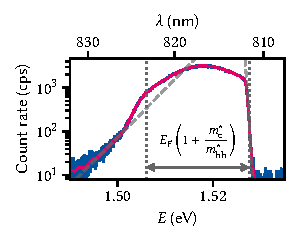
\includegraphics{img/pdf/experiment/2deg_pl}
    \caption[
        \sampleid{Doped M1_05_49-2}
        \thewavelength{795}
        \thepower{0.92}{\micro}
        \protect\newline
        \imgsource{img/py/experiment/pl.py}
    ]{
        \Gls{pl} of the bare \gls{2deg}.
        Magenta line is a smoothing spline fit to the data.
        Indicated by dotted gray lines are the Fermi edge at high and the band edge at low energy.
        The Fermi edge has a Fermi distribution (exponential indicated by a dashed gray line) whose temperature is typically much higher than the lattice temperature ($\sim\qty{1}{\kelvin}$).
        Below the band edge there is an exponential tail (dashed gray line) due to impurities that permeates far into the gap.
    }
    \label{fig:exp:pl:2deg}
\end{marginfigure}

\Cref{fig:exp:pl:2deg} shows a typical \gls{pl} spectrum obtained on the bare, unbiased \gls{qw} of a doped membrane sample.
This measurement corresponds to the configuration already discussed in \cref{sec:exp:theory:pl}.
Due to the Pauli exclusion principle, electrons require an energy of at least $E_\mr{F}\left(1 + m_{\mr{c}}^\ast/m_{\mr{hh}}^\ast\right)$ above the band gap and, because of the vanishingly small photon momentum, a momentum of at least $k_\mr{F}$ to be excited into a free state above the Fermi level $\mu$ (dotted gray line).\sidenote{
    This is known as the Burstein-Moss shift~\cite{Burstein1954,Moss1954}.
}
Once excited, they quickly relax down to the Fermi edge at $\mu$ from where they can recombine emitting a photon.
As the Fermi sea is at a finite temperature, the high-energy shoulder of the \gls{pl} spectrum is hence thermally broadened according to the Fermi distribution function of the electron gas (dashed gray line).
The associated temperature is around \qty{1.5}{\kelvin} and hence orders of magnitude higher than the lattice temperature of \qty{10}{\milli\kelvin}.
This effect has already been observed by \citet{Pinczuk1984}.
Like in those experiments, the temperature of the Fermi edge does not vary significantly with excitation power, making local heating of the lattice due to high excitation power an unlikely cause~\cite{Ulbrich1973}.
I show a power-dependence measurement of the Fermi edge supporting this statement in \cref{sec:app:exp:observations}.
\citet{Bockelmann1990} showed that in low-dimensional electron gases electron cooling by phonon emission is limited by a finite scattering rate.
Thus, under continuous excitation a quasi-equilibrium is established as hot electrons cannot loose heat quickly enough.
Although their simulations were performed for higher temperatures and smaller confinement widths, their results of electron temperatures in the range of \qty{2}{\kelvin} for lattice temperatures of \qty{300}{\milli\kelvin} is comparable to ours.

\Gls{pl} emission is possible also at lower energies as electrons inside the Fermi sea recombine with the free photo-hole that scatters towards the valence band ege.
The band gap then defines the low-energy shoulder of the \gls{pl} spectrum, below which there are -- ideally -- no states available (dotted gray line).
However, the \gls{pl} reveals there are indeed free states decaying exponentially into the gap, originating most likely from impurities (dashed gray line).
Compared to the results of \citet{Kamburov2017}, the \gls{pl} spectra obtained here are much flatter over energy, with the \gls{pl} peak typically close to the middle between gap and Fermi edge.
Conversely, \citet{Kamburov2017} observed a strong peak at the band gap,\sidenote{
    \Cf also \citet{Gabbay2008}, who observe all but no \gls{fes} in samples nominally comparable to ours.
}
indicating that in our samples holes are more strongly localized and therefore have a wider spread in $k$-space, enabling transitions in a wider range of wave vectors~\cite{Skolnick1987}.
This would in turn imply increased alloy disorder or interface roughness~\cite{Gabbay2008}, an observation we shall come back to in \cref{sec:exp:observations:ple}.

From the width of the \gls{2deg} emission, we can calculate the charge carrier density by relating it to the Fermi energy in two dimensions~\cite{Pinczuk1984,Ihn2009},
\begin{equation}\label{eq:exp:pl:n}
    n = \frac{m^{\ast}_{\mr{c}}E_{\mr{F}}}{\pi\hbar^2} = \frac{\mu\Delta E}{\pi\hbar^2},
\end{equation}
where $\Delta E$ is the bandwidth of the emission (dashed gray lines in \cref{fig:exp:pl:2deg}) and $\mu = m^{\ast}_{\mr{c}}m^{\ast}_{\mr{hh}}/(m^{\ast}_{\mr{c}} + m^{\ast}_{\mr{hh}})$ is the reduced mass of conduction and valence band.
For this particular sample, \cref{eq:exp:pl:n} yields $n = \qty{5e11}{\per\square\centi\meter}$ or, equivalently, $E_{\mr{F}} = \qty{18}{\milli\electronvolt}$ and $k_{\mr{F}} = \qty{1.8e8}{\per\meter}$.
Comparing this value to that obtained from a simulation of the heterostructure with nominal doping concentration $N_{\mr{d}} = \qty{6.5e17}{\per\cubic\centi\meter}$ using a self-consistent Poisson-Schrödinger solver~\cite{PoissonSchroedinger}, $n = \qty{1.9e11}{\per\square\centi\meter}$ (refer to \cref{sec:app:exp:observations} for simulation parameters), shows a significant discrepancy indicating a severe mismatch between nominal and actual doping concentrations.\sidenote{
    Note that the carrier density obtained thus does not vary significantly with excitation power, ruling out photo-doping as a source of the discrepancy.
    See \cref{sec:app:exp:observations} for a measurement of the \gls{2deg} \gls{pl} as function of power.
}
Finally, we observe that the gap according to the preceding analysis is redshifted from the undoped bulk gap of \qty{1.519}{\electronvolt}~\cite{Vurgaftman2001} by \qty{13}{\milli\electronvolt}.\sidenote{
    The redshift is in fact larger still due to the confinement energy of the \gls{qw}, estimated to be $\qty{17}{\milli\electronvolt}$ in \cref{sec:exp:theory:qcse}.
}
\Citet{Descamps2021} hypothesized that the removal of the \ch{GaAs} substrate and the associated change in strain leads to this lowering of the band gap.
However, this effect was also already observed by \citet{Pinczuk1984} in \enquote{bulk} modulation-doped \ch{GaAs} \glspl{qw}.
There, the authors put forth a renormalization of the band gap due to many-body interactions as an explanation, an interpretation since well-agreed upon~\cite{Jain1992}

\subsection{Quantum-confined Stark shift}\label{subsec:exp:observations:pl:qcse}

\begin{figure}
    \centering
    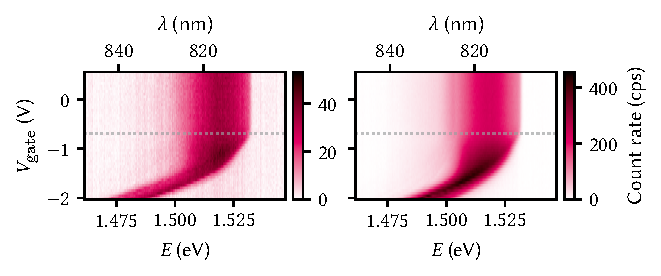
\includegraphics{img/pdf/experiment/honey_H13_stark_shift_vs_gate}
    \caption[
        \sampleid{Honey H13}
        \thewavelength{795}
        \thepower{1}{\micro}
        \protect\newline
        \imgsource{img/py/experiment/pl.py}
    ]{
        \Gls{pl} as function of gate voltage on a single fan-out gate on the bottom (left) and top (right) side of the membrane.
        The behavior is qualitatively similar but the overall quantum efficiency lower by an order of magnitude for gates on the bottom (as-grown buried) side.
        Dotted gray lines are a guide to the eye demonstrating that the changes to the \gls{pl} spectrum set in at the same voltage for both types of gates (around \qty{-0.7}{\volt}).
    }
    \label{fig:exp:pl:honey_H13_stark_shift_vs_gate}
\end{figure}

Let us now address the behavior of the \gls{pl} under electric fields.
To this end, the laser is positioned on an \gls{ebl}-written gate and a negative voltage is applied to the gate.
\cref{fig:exp:pl:honey_H13_stark_shift_vs_gate} depicts two measurements on a well-behaved sample.
The left (right) panel shows the \gls{pl} as function of voltage with the laser positioned on a bottom (top) gate.
In contrast to the intuition obtained in \cref{sec:exp:theory:qcse}, there is no immediate effect to be observed once the voltage is switched on.
This is most likely due to the presence of the \gls{2deg} screening the external electric field. % TODO: look at literature
At $V_{\mr{gate}} = \qty{-0.7}{\volt}$, the high-energy shoulder of the emission starts to shift towards lower energies while the low-energy shoulder stays invariant.
Per the previous section, we can interpret this as the charge carrier density and thereby the Fermi energy being lowered as the \gls{2deg} is depleted.
As the electric field tilts the bands, the band edges of both conduction and valence band shift by the same amount and therefore the band gap is not modified in this regime.\sidenote{
    We would in fact expect a slight increase in confimenent energy as the carrier density is lowered because the band bending due to the surplus electric charge of the \gls{2deg} is lifted.
}
As the \gls{2deg} is gradually depleted, a broad exciton peak emerges that shifts approximately quadratically with the applied voltage as ionization from the interaction with the Fermi sea of electrons becomes less pronounced (\cf \cref{sec:exp:theory:pl}).
Beyond \qty{-1.5}{\volt}, the \gls{2deg} is completely depleted.
The voltage difference between onset and completion of the depletion matches roughly the value expected from a simulation without screening for the nominal device parameters (see \cref{tab:app:exp:samples,tab:app:exp:samples:ps}), \qty{-0.7}{\volt}.

Besides the voltage dependence, another feature stands out from \cref{fig:exp:pl:honey_H13_stark_shift_vs_gate}: the \gls{pl} intensity is lower by an order of magnitude when on top of a back gate compared to a top gate.
This is at first puzzling, as in the latter case there is an additional semi-transparent gate\sidenote{
    \qty{7}{\nano\meter} \ch{Au} with a \qty{2}{\nano\meter} \ch{Ti} adhesion layer.
}
absorbing and reflecting both laser and \gls{pl} radiation, whereas in the former there is only the bare heterostructure, so we would expect the exact opposite!
I elucidate this issue in \cref{sec:exp:tmm}.

\begin{marginfigure}
    \centering
    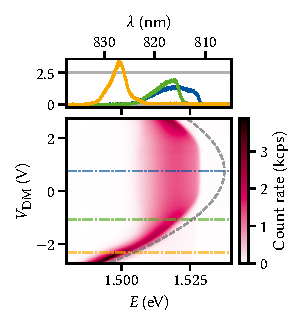
\includegraphics{img/pdf/experiment/doped_M1_05_49-2_difference_mode}
    \caption[
        \sampleid{Doped M1_05_49-2}
        \thevoltage{-1.3}{CM}
        \thewavelength{795}
        \thepower{10}{\micro}
        \protect\newline
        \imgsource{img/py/experiment/pl.py}
    ]{
        \Gls{pl} as function of difference-mode voltage on a large exciton trap.
        The observed Stark shift follows roughly the expected quadratic dispersion, but is offset by \qty{0.75}{\volt} with respect to zero bias.
        Dashed gray line is a guide to the eye of a parabola with curvature \qty{-3.5}{\milli\electronvolt\per\volt\squared}.
        Line cuts in the upper panel are taken at the voltages indicated by dash-dotted lines in the lower, and arrows indicate positions of individual peaks making up the yellow line shape.
    }
    \label{fig:exp:pl:doped_M1_05_49-2_difference_mode}
\end{marginfigure}

Moving to a large exciton trap with a single set of top and bottom gates and \qty{5}{\micro\meter} diameter, we can measure the behavior of the Stark shift in the intended setting of local confining gates on either side of the membrane.
We define the virtual gates
\begin{align}\label{eq:exp:observations:virtual_gates}
    \VDM &= \VT - \VB, \\
    \VCM &= \VT + \VB,
\end{align}
where DM (CM) stands for difference (common) mode and T (B) for top and bottom, respectively.
Clearly, \VDM should ideally be proportional to the out-of-plane electric field across the membrane, $\VDM = Ft$ with $t$ the membrane thickness, whereas \VCM should tune the band edge offset from the Fermi level $\mu$.
As we observed previously, the presence of the \gls{2deg} screens the electric field generated by \VDM.
A good operating point is therefore at a negative \VCM which should deplete the \gls{2deg} (or at least reduce the charge carrier density).
\Cref{fig:exp:pl:doped_M1_05_49-2_difference_mode} shows a \gls{pl} map as function of the difference mode voltage \VDM at $\VCM = \qty{-1.3}{\volt}$.
From \cref{fig:exp:pl:honey_H13_stark_shift_vs_gate}, where the optical measurement of the charge carrier density results in a similar value as for the sample in \cref{fig:exp:pl:doped_M1_05_49-2_difference_mode}, $n\sim\qty{5e11}{\per\centi\meter\squared}$, we would expect this common mode voltage to suffice in at least overcoming the screening and reducing the carrier density in the \gls{qw}.
However, there is clearly still \gls{2deg} emission present for a large range of \VDM, and the Fermi edge is at the same energy as without a gate bias.
Overall, the Stark shift pattern is symmetric but offset by $\VDM = \qty{0.75}{\volt}$.
This behavior is also observed in the response of the \gls{pl} to a single gate in this and several other samples, where the onset of an effect by bottom gate is significantly later than that for the top gate, suggesting that the voltage is screened by some mechanism and the bottom gate has a much smaller lever arm than the top gate.
Perhaps surprisingly, the gates on the \emph{bottom} side of the membrane display this behavior, \ie, the gates on the as-grown surface.\sidenote{
    I note that the sample of \cref{fig:exp:pl:honey_H13_stark_shift_vs_gate} was fabricated on the same heterostructure as the device in Figure 4(d) of \citer{Descamps2023}, which showed little to no electrical hysteresis unlike most other samples investigated by \citet{Descamps2021}.
}
This makes surface states an unlikely candidate for the screening as the quality of the grown surface should be better than that of the etched surface~\cite{Descamps2021}.
A possible cause might be oxygen segregation during growth\sidenote{A.~Ludwig, private communication.} or other impurities~\cite{Nguyen2020}.

The fact that the \gls{2deg} is depleted by \VDM in the range \qtyrange{-0.2}{-1.4}{\volt} and above \qty{1.5}{\volt} at all is unexpected.
Even with a difference in lever arms as just discussed, the symmetric dependence of the \gls{pl} emission on \VDM implies that $\VDM - \qty{0.75}{\volt}$ \emph{should} correspond to the out-of-plane electric field such that the energy is unchanged in the middle of the quantum well, $\VDM - \qty{0.75}{\volt} \propto F(z-t/2)$.
Staying in the virtual gate picture, a difference in relative lever arms\sidenote{
    Relative gate lever arms are unitless parameters used to quantify the degree of cross-coupling between gates, in contrast to the physical lever arms used to quantify the change in electron energy versus gate voltage employed in \cref{sec:setup:cooling:etemp}.
    See for example \citer{Volk2019}.
}
$\Delta\alpha = \alpha_{\mr{T}} - \alpha_{\mr{B}}$ between \VT and \VB should modify the virtual gates as
\begin{align}\label{eq:exp:virtual_gates}
    \begin{pmatrix}
        \tilde{V}_{\mr{DM}} \\
        \tilde{V}_{\mr{CM}}
    \end{pmatrix}
    &= \frac{1}{\sqrt{1 + \Delta\alpha^2}}\begin{pmatrix}
        1 & \Delta\alpha \\
        -\Delta\alpha & 1
    \end{pmatrix}\begin{pmatrix}
        \VDM \\
        \VCM
    \end{pmatrix} \\
    &= \frac{1}{\sqrt{1 + \Delta\alpha^2}}\begin{pmatrix}
        1 + \Delta\alpha & -1 + \Delta\alpha \\
         1 - \Delta\alpha & 1 + \Delta\alpha
    \end{pmatrix}\begin{pmatrix}
        \VT \\
        \VB
    \end{pmatrix}
\end{align}
and as such not modify the qualitative behavior of \VDM besides the offset.\sidenote{
    Setting $\Delta\alpha = \num{0.6}$ yields a $\tilde{V}_{\mr{DM}}$ for which the Stark shift in \cref{fig:exp:pl:doped_M1_05_49-2_difference_mode} is symmetric about zero.
}
That is, in and of itself, \VDM should not reduce the charge carrier density in an isolated \gls{qw} to first order.\sidenote{
    We might instead expect a small change in the apparent gap energy as the well is tilted.
}

One possible explanation for the observed behavior is the depletion of the \gls{2deg} by electrons tunneling out of the well and recombining with the donor ions, rendering one of the doped barriers electrically neutral.
With the doping pulling down the conduction band between \qty{50}{\nano\meter} and \qty{90}{\nano\meter} away from the \gls{qw}, the tunneling rate will be more pronounced than estimated for the undoped case in \cref{sec:exp:theory:qcse}.
Taking the large trap diameter in this case into account, there are $\sim\num{1e5}$ electrons in the unbiased \gls{qw} on the area of the trap gates.
Thus, at a tunneling rate of \qty{1}{\mega\hertz}, all electrons would tunnel out of the \gls{qw} within \qty{100}{\milli\second} on average, putting a response of the system into the steady state within the fairly long time scales of a \gls{pl} measurement\sidenote{
    Say \qtyrange{0.1}{10}{\second}.
}
well within reasonable bounds.
In the literature, this is known as carrier sweep-out and has been studied in the context of solar cells and other electroabsorptive devices~\cite{Larsson1988,Schneider1988,Fox1991}.

The dashed gray line in \cref{fig:exp:pl:doped_M1_05_49-2_difference_mode} shows a parabola, $\Delta E\propto \alpha\VDM^2$, with curvature $\alpha = \qty{-3.5}{\milli\electronvolt\per\volt\squared}$ as a guide to the eye.
For difference-mode voltages below \qty{-1.8}{\volt}, the exciton Stark shift follows this quite closely, establishing that the exciton energy can be tuned by over \qty{20}{\milli\electronvolt} in the depleted regime, which simulations suggest is sufficient for confinement of single excitons in a smaller trap geometry~\cite{Descamps2021}.
The upper panel depicts three line cuts at the positions indicated by the dash-dotted lines in the main panel.
As can be seen from the cut at \qty{-2.3}{\volt} (orange), the line shape appears to consist of three individual emission lines assigned by \citet{Descamps2021} as the neutral, singly, and doubly negatively charged excitons. % TODO: exciton/trion mixing ref
I return to the question of line assignment below.

\subsection{Power dependence}\label{subsec:exp:observations:pl:power}
\begin{figure}
    \centering
    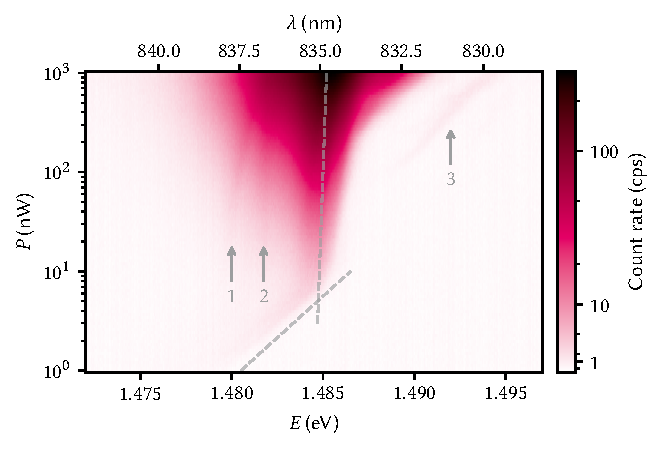
\includegraphics{img/pdf/experiment/doped_M1_05_49-2_power}
    \caption[
        \sampleid{Doped M1_05_49-2}
        \thevoltage{-2.7}{DM}
        \thevoltage{-1.3}{CM}
        \thewavelength{795}
        \protect\newline
        \imgsource{img/py/experiment/pl.py}
    ]{
        \Gls{pl} as function of excitation power $P$.
        In the left panel two qualitatively different regimes are indicated by dashed gray lines as guides to the eye; below \qty{10}{\nano\watt}, the main peak displays a blueshift logarithmic in excitation power, $E = \qty{1.485}{\electronvolt} + \qty{5}{\milli\electronvolt}\log_{10} P$.
        Above, the blueshift diminishes significantly.
        Three additional lines, indicated by arrows, with varying power dispersion are visible.
        Right panel shows a fit to data at $P=\qty{1}{\micro\watt}$.
        A sum of seven individual lines (dashed, gray) is required to fit the data.
        The dashed gray lines are the individual contributions.
    }
    \label{fig:exp:pl:doped_M1_05_49-2_power}
\end{figure}

As outlined in \cref{sec:exp:theory:complexes}, the dependence of emitted \gls{pl} power on excitation power of individual emission lines can help inferring the excitonic species responsible.
Moreover, as the density of excitons depends on the excitation power, interaction effects between them influence the energy of the emission.
Such a measurement is shown in the left panel of \cref{fig:exp:pl:doped_M1_05_49-2_power} for the same common-mode voltage as in \cref{fig:exp:pl:doped_M1_05_49-2_difference_mode} and $\VDM = \qty{-2.7}{\volt}$ (\ie, corresponding to the lowest line in that plot) where the \gls{2deg} is completely depleted.
Two qualitatively different regimes can be observed as indicated by the dashed gray lines as guides to the eye.
Below \qty{10}{\nano\watt} excitation power, corresponding to approximately \qty{0.75}{\watt\per\square\centi\meter} at the beam diameter measured in \cref{part:setup}, the main line displays a blueshift logarithmic in excitation power.
Above this value, the blueshift is much less pronounced.
It is not understood though why the blueshift abruptly changes in quality at \qty{10}{\nano\watt} excitation power.
At powers above \qty{10}{\nano\watt}, two additional lines on the low-energy side of the main peak become visible that appear to converge towards higher powers, while above \qty{100}{\nano\watt} a line appears on the high-energy side that has a similar blueshift as the main peak at low powers.
In principle, the blueshift as function of power is to be expected.
Increasing the excitation power increases the density of excitons, either because they are spatially localized or because of a finite diffusion speed.
The increased density corresponds to an increased overlap of single excitons' constituents and thus in turn leads to an increasingly repulsive Coulomb interaction that raises their energy.\sidenote{
    Of course, the opposite -- an attractive interaction -- is also possible for small numbers of excitons, resulting in biexcitons.
    The two cases can be thought of analagously as bonding and anti-bonding orbital configurations.
}
This mechanism underpins the use of exciton traps such as \glspl{saqd} as single-photon sources; upon spectrally filtering on the emission wavelength of a single exciton, only a single photon can be emitted from the trap at a time since the presence of another exciton in the trap would shift the emission energy of both. % TODO: move this somewhere else?

The right panel shows a line cut taken at \qty{1}{\micro\watt}.
A weighted sum of seven individual Voigt profile line shapes~\cite{VoigtProfileWiki},
\begin{subequations}\label{eq:exp:voigt}
    \begin{equation}\tag{\ref{eq:exp:voigt}}
        V(E; \sigma, \gamma) = G(E; \sigma) \ast L(E; \gamma),
    \end{equation}
    that is, a convolution of Gaussian and Lorentzian line shapes given by
    \begin{align}
        G(x; \sigma) &= \frac{1}{\sigma\sqrt{2\pi}}\exp(-\frac{x^2}{2\sigma^2}), \label{eq:exp:gaussian} \\
        L(x; \gamma) &= \frac{1}{\pi}\frac{\gamma}{\gamma^2 + x^2}, \label{eq:exp:lorentzian}
    \end{align}
\end{subequations}
is required to obtain an adequate fit.
The Voigt profile arises from a combination of two separate line broadening mechanisms that manifest as a Gaussian (\cref{eq:exp:gaussian}) and Lorentzian (\cref{eq:exp:lorentzian}) line shape.
The former describes inhomogeneous broadening due to noise faster than the data acquisition time, whereas the latter is the homogeneous broadening due to for example the finite lifetime of the emitting state\sidenote{
    This is also known as the linewidth's transform limit; energy and (life)time are Fourier pairs by Heisenberg's uncertainty principle.
}
or power broadening~\cite{Citron1977}.
All but the two outermost lines in the best fit are dominated by the inhomogeneous, Gaussian contribution to \cref{eq:exp:voigt} with widths $\sigma$ in the range of \qtyrange{0.1}{1}{\milli\electronvolt} and a peak separation on the order of \qty{2}{\milli\electronvolt}.\sidenote{
    The large number of Voigt profiles used to fit the data does tend to overfit the data.
}

According to \citer{Descamps2021}, the lifetime of a Stark-shifted exciton is on the order of \qty{1}{\nano\second} due to the reduced wave function overlap.
This corresponds to a homogeneous linewidth of $2\gamma = \flatfrac{\hbar}{\tau} \sim \qty{660}{\nano\electronvolt}$, several orders of magnitude below the observed linewidth, and it is thus consistent with the fact that most peaks are best fit by inhomogeneously broadened line shapes.
This large a number of lines is certainly unexpected and cannot be explained by different excitonic species.
Where it is possible to track individual peaks as function of excitation power, their power dependence is linear, $\int\dd{E} V(E)\propto P$, suggesting neutral excitons or band-to-band recombination as origins of the emission.

\begin{figure*}
    \centering
    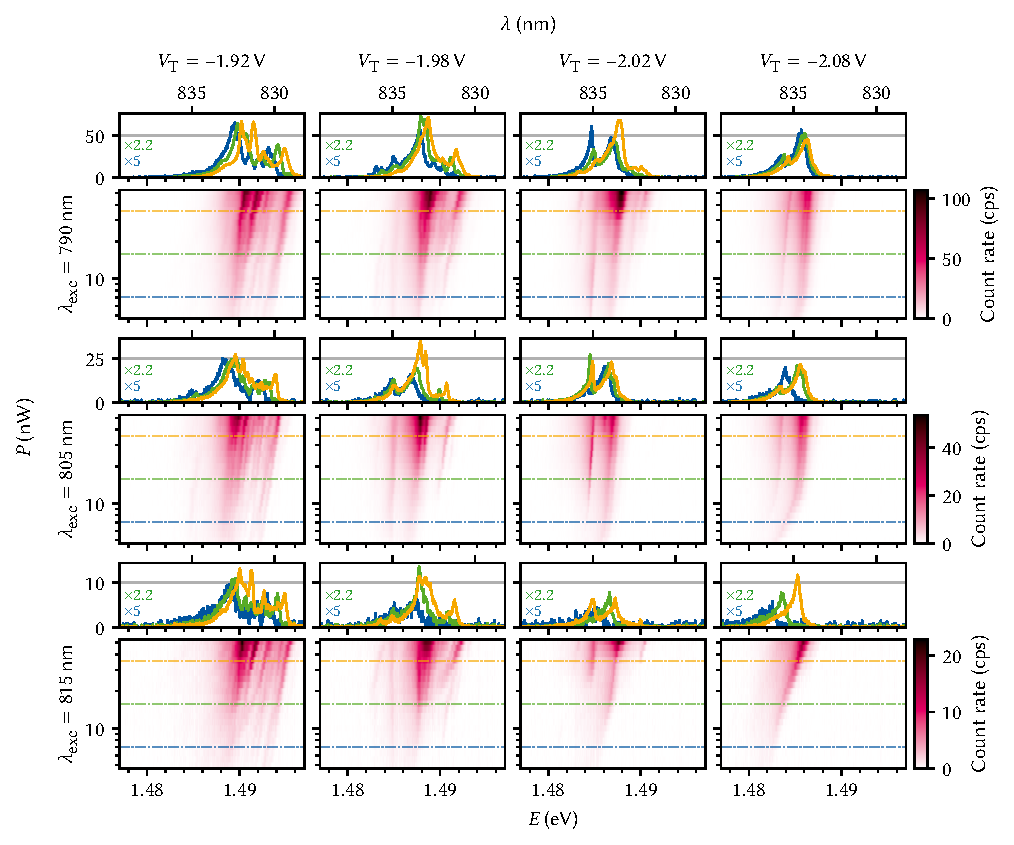
\includegraphics{img/pdf/experiment/doped_M1_05_49-2_multiplets}
    \caption[
        \sampleid{Doped M1_05_49-2}
        \thevoltage{0}{B}
        \protect\newline
        \imgsource{img/py/experiment/pl.py}
    ]{
        Wide-range \gls{pl} parameter sweep on a large exciton trap plotted as function of excitation power and detection energy.
        Rows are data for three different excitation wavelengths, columns for four different top gate voltages \VT and share color and line cut scales.
        Line cuts are taken at the indicated positions of $P_{\mathrm{det}} = \qtylist{7;16;35}{\nano\watt}$ and drawn scaled by the fraction of excitation power with respect to \qty{35}{\nano\watt}.
    % Atomic step fluctuations would shift by ~900 μeV (a = 5.6 Α)
    }
    \label{fig:exp:pl:doped_M1_05_49-2_multiplets}
\end{figure*}

A possible explanation for the multitude of lines is thus that they originate from different spatial locations, a hypothesis we return to shortly.
First, let let us conclude this section with a large parameter sweep of this trap, shown in \cref{fig:exp:pl:doped_M1_05_49-2_multiplets}.
Each of the three rows (with separate panels for line cuts each) show data for different excitation wavelengths, $\lambda_{\mr{exc}}$, each of the columns show data for different top gate voltage, \VT, and the \gls{pl} is plotted as function of detection energy, $E_{\mr{det}}$, and excitation power, $P_{\mr{exc}}$.
The line cuts taken at lower powers (blue and green) are scaled to match the one at the highest power (orange) assuming a linear power dependence.
For all data $\VB = \qty{0}{\volt}$ so that $\VT = \VDM = \VCM$.
Despite the comparatively small changes in voltage, the behavior of the sample changes significantly.
Whereas for $\VT = \qty{-2.08}{\volt}$ the observed \gls{pl} features are similar to those in \cref{fig:app:exp:observations:2deg_pl_power_dependence},
at $\VT = \qty{-1.92}{\volt}$ there is a very large number of lines in the spectrum, most but not all of which share the same blueshift as function of excitation power.
The effect of a different excitation wavelength appears to mostly be a shift of the features along the excitation power axis and thus simply a change in absorption efficiency, although some features also change qualitatively.
I discuss the wavelength dependence in more detail in \cref{sec:exp:observations:ple}.

So what is the origin of the substructure of the \gls{pl} emission?
The peak distance is on the order of \qty{1}{\milli\electronvolt}.
This value is on the order of magnitude of the change in ground state energy, \qty{470}{\micro\electronvolt}, we would expect from fluctuations in the width of the \gls{qw} by one atomic layer of \ch{GaAs} with lattice constant $a = \qty{5.65}{\angstrom}$\sidenote{
    Meaning the thickness of a single atomic layer is $a/2$.
}
for the design well width $L = \qty{20}{\nano\meter}$ (\cref{sec:exp:theory:pl}).
Indeed, there exists a large body of literature that has examined the influence of interface roughness and \gls{qw} thickness fluctuations on the exciton \gls{pl}~\cite{Tanaka1987,Gammon1991,Leosson2000}.
Not only do atomic steps and islands lead to increased \gls{pl} linewidth and energy shifts, but in fact also to the possible localization of single excitons~\cite{Brunner1994,Brunner1994a,Zrenner1994}.
That is to say, \glspl{qd} have been found to form at such interface fluctuations.
Comparing the spectra shown in \cref{fig:exp:pl:doped_M1_05_49-2_multiplets} to those shown by \citet[Figure~1]{Brunner1994}, our main \gls{pl} line is more reminiscent of what the authors there label as the 2D exciton; our spectra do not show well-separated and sharp lines on the low-energy side of the spectrum.
By contrast, the \gls{pl} spectrum shown by \citet[Figure~1]{Zrenner1994} is very similar to the one observed here, although they assign this peak to indirect transitions from the \ch{AlAs} $X$ valley to the \ch{GaAs} $\Gamma$ valence band valley in their \ch{AlAs/GaAs} coupled \gls{qw} structure, a situation quite unlike ours.

An intricate substructure of the \gls{pl} emission at lower excitation powers such as this was also observed in other samples.
If the individual lines originated from 0D-confined \glspl{qd}, we would expect their \gls{pl} emission to display signatures of a single-photon source as outlined above. % TODO: "above"
I therefore performed a \g2 measurement (see \cref{sec:setup:optics:g2}) on a line that was narrow ($\sim\qty{1}{\milli\electronvolt}$) and fairly well-separated such that at its \gls{fwhm} was resolvable.
I excited the sample above the gap and spectrally filtered the emitted \gls{pl} by using the spectrometer as a monochromator with bandwidth given by the line \gls{fwhm}.
Due to the low brightness, a compromise between high excitation power (leading to power broadening) and measurement duration (to gather statistics) was chosen at \qty{100}{\nano\watt}.
However, after \qty{48}{\hour} no deviation from a flat and uncorrelated \g2 could be observed.\sidenote{
    I also attempted a \g2 measurement to no avail in a different parameter regime where a single, isolated emission line appears.
    % TODO: #218; expand, show data?
}

\subsection{Spatial dependence}\label{subsec:exp:observations:pl:spatial}
\begin{marginfigure}
    \centering
    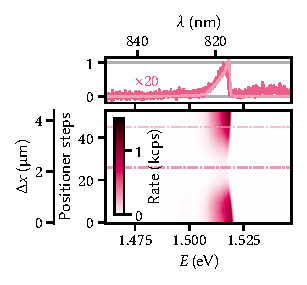
\includegraphics{img/pdf/experiment/fig_F10_positioning}
    \caption[
        \sampleid{Fig F10}
        \thewavelength{795}
        $V_{y}=\qty{30}{\volt}$
        \protect\newline
        \imgsource{img/py/experiment/pl.py}
    ]{
        \Gls{pl} of the unbiased \gls{qw} as the laser is stepped across a bottom gate.
        The line traces in the upper panel are taken at the positions indicated by dash-dotted lines.
        Positioner steps are converted to distance using a linear fit of the positioner readout after the initial hysteresis has worn off (about \num{10} steps).
        The Fermi edge shows a slight redshift when on top of the gate in this sample.
    }
    \label{fig:exp:pl:fig_F10_positioning}
\end{marginfigure}

As mentioned several times already, the nanopositioners on which the sample is mounted show hysteresis and are therefore not suited for reproducible spatial maps of the sample.
The hysteresis is due to the non-adiabaticity of the method of movement in the so-called slip-stick mode (\cf \cref{ch:setup:cooling}).
What is more, the resistive position readout is also fairly unreliable below, say, \qty{5}{\micro\meter} resolution.
Nonetheless, we can at the very least perform simple one-dimensional sweeps after manually positioning the sample at a given starting position and assume that the displacement per step has some sufficiently narrow distribution around a fixed mean.
A more sophisticated algorithmic approach using feature detection may allow also two-dimensional maps with a reasonable accuracy.

\Cref{fig:exp:pl:fig_F10_positioning} shows the \gls{pl} collected from the sample as the positioner is stepped perpendicularly across an unbiased gate.
The vertical axis also gives a position coordinate which is computed from the steps by fitting the position readout once hysteresis has worn off.
The blue and green dash-dotted line correspond to the center of and beside the gate, respectively, with line cuts drawn in the upper panel.
Clearly, the \gls{pl} intensity is quenched significantly by the gate, beyond what one could expect from simple reflection and absorption of laser and \gls{pl} radiation.
I perform \gls{tmm} simulations to explain this behavior in \cref{sec:exp:tmm} (see also \cref{fig:exp:pl:honey_H13_stark_shift_vs_gate}).
Curiously, the map also shows a shifting of the Fermi edge close to the gate.
This behavior was observed consistently on this sample next to an unusual \gls{pl} line shape (\cf \cref{fig:exp:pl:2deg}).
The former effect could potentially be caused by band-deformation due to strain from the metallic gates.

\begin{marginfigure}
    \centering
    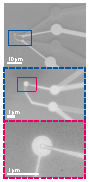
\includegraphics{img/pdf/experiment/sem}
    \caption[\imgsource{img/py/experiment/sem.py}]{
        \acrshort{sem} image of an exciton trap with both central and guard gates.
        Gates on the bottom side are visible through the membrane.
        Positions (symbolic) of the line cuts in \cref{fig:exp:pl:doped_M1_05_49-2_positioning} are indicated in the same colors.
        Images taken by Thomas Descamps.
    }
    \label{fig:exp:pl:sem}
\end{marginfigure}

\begin{figure}
    \centering
    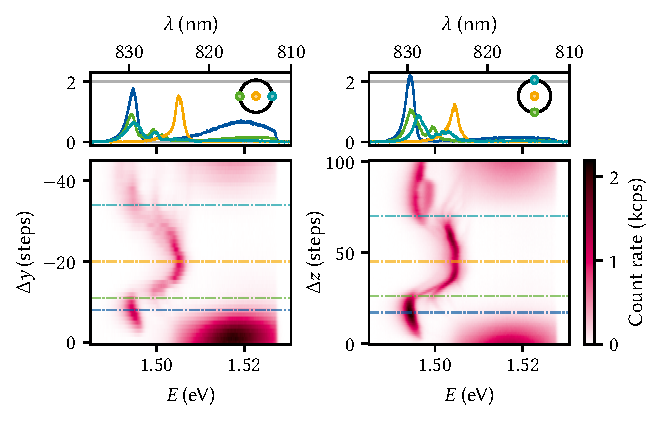
\includegraphics{img/pdf/experiment/doped_M1_05_49-2_positioning}
    \caption[
        \sampleid{Doped M1_05_49-2}
        \thevoltage{-0.43}{DM}
        \thevoltage{-3.75}{CM}
        $V_{y}=V_{z}=\qty{30}{\volt}$.
        \thepower{1}{\micro}
        \thewavelength{795}
        \protect\newline
        \imgsource{img/py/experiment/pl.py}
    ]{
        \Gls{pl} of a large exciton trap as function of position perpendicular (left) and parallel (right) to gravity.
        The trap is biased so that the emission is Stark-shifted towards lower energy.
        Upper panels show line cuts taken along the dash-dotted lines in the lower panels, demonstrating fairly identical behavior along both axes.
        The cuts in orange, green, and teal are taken at positions corresponding to the ones marked in the bottom panel of \cref{fig:exp:pl:sem}, with orange corresponding to the center of the trap gate.
    }
    \label{fig:exp:pl:doped_M1_05_49-2_positioning}
\end{figure}

\Cref{fig:exp:pl:doped_M1_05_49-2_positioning} shows two sweeps along orthogonal axes across the biased large exciton trap with a single gate discussed before in \cref{fig:exp:pl:doped_M1_05_49-2_difference_mode,fig:exp:pl:doped_M1_05_49-2_power,fig:exp:pl:doped_M1_05_49-2_multiplets}.
While this is not unequivocal proof of zero-dimensional confinement, it does suggest that the effective exciton potential is laterally lowered.
The left panel of \cref{fig:exp:pl:doped_M1_05_49-2_positioning} shows a scan along the in-plane axis perpendicular to gravity, while the right shows the in-plane axis parallel and against gravity.
Regrettably, the resistive position readout did not yield anything but noise in these measurements, prohibiting a conversion of positioner steps into relative position as before.
Both scans were acquired with the sample voltage applied to the positioners (\qty{30}{\volt}), which is the same used in \cref{fig:exp:pl:fig_F10_positioning} as well.
We can hence roughly expect \num{10} steps to correspond to \qty{1}{\micro\meter} in $y$ direction.
Naturally, a single step against gravity displaces the sample by a smaller amount compared to the perpendicular direction, but given the circular shape of the trap and the similarity of the \gls{pl} features, the displayed ranges should be roughly the same.
The upper panels show line cuts taken at the positions indicated by dash-dotted lines in the lower panels, with the orange, green, and teal lines corresponding to the positions indicated by markers on a different trap in \cref{fig:exp:pl:sem}.
Both sweeps display very similar features.
In the center of the trap (yellow), the Stark-shifted emission line consists of a single peak.
Towards the edges (teal and green), two surprising effects take place: first, the Stark shift of the dominant peak increases in magnitude, and second, a large number of additional, faint lines appear.
The increase in effective electric field towards the edge of an exciton trap is reminiscent of the simulation of the same type of experiment for an undoped \gls{qw} by \citet[Figure~6.4]{Descamps2021}, although it was not explained there.
Indeed, it also appears to be in conflict with Figure~2.16 \ibid, where a monotonic increase in effective exciton potential as function of distance from the trap center was predicted.
In the device under study here, there is of course a \gls{2deg} whose presence towards the edge of the trap screens the voltages, in theory contributing to an attenuation of the Stark shift.
Why we observe to opposite is thus quite puzzling.

The second surprising feature seen in \cref{fig:exp:pl:doped_M1_05_49-2_positioning} is the addition of faint lines that appear to branch out from the main exciton line as the laser spot is moved away from the center of the trap.
These could be related to the lines observed in \cref{fig:exp:pl:doped_M1_05_49-2_multiplets} as well as the large number of lines required to fit the peak in \cref{fig:exp:pl:doped_M1_05_49-2_power}.
If the origin of these are indeed atomic steps or islands in the \gls{qw}, it makes sense that we observe them in these measurements.
The Stark shift of the different lines appears depend on the position as well, indicating different coupling to the electric field and further strengthening the hypothesis that they originate from different spatial locations.

\section{Photoluminescence excitation spectroscopy}\label{sec:exp:observations:ple}
The technique of \acrfull{ple} can be used to gain insight into the energy level structure of optically active states~\cite{Gilliland1997}.
While in a \gls{pl} experiment we only observe the emission, \gls{ple} experiments are sensitive to absorption as well.
Thus, excited states that quickly decay non-radiatively before recombining can be probed as absorption at that energy will be enhanced even though emission might not.
For well-resolved \gls{pl} lines, a common practice is to spectrally filter the \gls{pl} radiation while sweeping the excitation laser wavelength, thus obtaining the luminescence intensity as function of excitation energy, $I_{\mr{PLE}}(E_{\mr{exc}}; E_{\mr{det}})$, for a single detection energy $E_{\mr{det}}$.
By contrast, a \gls{pl} measurement is performed at a fixed excitation energy and yields $I_{\mr{PL}}(E_{\mr{det}}; E_{\mr{exc}})$.
Alternatively, the entire \gls{pl} spectrum can be integrated up to the excitation energy rather than filtered at specific energy,
\begin{equation}\label{eq:exp:ple}
    I(E_{\mr{exc}}) = \int_{0}^{E_{\mr{exc}}}\dd{E_{\mr{det}}} I(E_{\mr{det}}, E_{\mr{exc}}),
\end{equation}
which yields a better \gls{snr} at the cost of potentially washing out selective transitions.

What do we expect for the \gls{ple} of a \gls{qw} hosting a \gls{2deg}?
By Fermi's exclusion principle, no free states are available below the Fermi level $\mu$ and thus excitation of an electron-hole pair from the valence band into the conduction band is only possible for photon energies above $E_{\mr{F}}(1 + m_{\mr{c}}^\ast/m_{\mr{hh}}^\ast)$ (\cref{sec:exp:theory:pl}).
Accordingly, the \gls{ple} spectrum should show an onset at that energy.\sidenote{
    In fact, the \gls{fes} should lead to a peak at the onset of the spectrum.
}
Above it, there exists a continuum of states in the \gls{qw} plane, and the \gls{ple} spectrum should remain approximately constant until higher-lying states can be reached.
In a single \gls{qw}, these can be either higher subbands of heavy-hole valence or conduction bands or indeed light-hole transitions due to heavy-hole--light-hole mixing~\cite{Bastard1984,Miller1985b,Laruelle1988,Reynolds1988,ElKhalifi1989}.
For the relatively wide \gls{qw} widths in our samples, we would expect the latter to be on the order of a few \unit{\milli\electronvolt}.

Applying an external electric field should further enhance the light-hole transitions as tilting the \gls{qw} breaks the symmetry forbidding light-hole transitions~\cite{Collins1986,Collins1987}.
Furthermore, the electric field depletes the \gls{2deg} as we have seen in \cref{fig:exp:pl:doped_M1_05_49-2_difference_mode} and should result in a laterally local potential well for excitons with discrete and approximately equidistant energy levels as laid out in \cref{subsec:exp:theory:qcse:trap}.
If such were the case, we would expect resonances in the \gls{ple} at intervals corresponding to the level spacing $\hbar\omega$ of the potential well that would confirm 0D-confinement.

\begin{figure}[H]
    \centering
    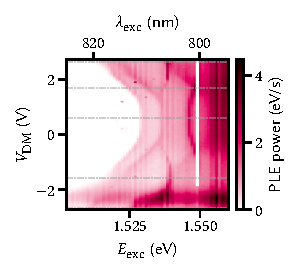
\includegraphics{img/pdf/experiment/doped_M1_05_49-2_ple}
    \caption[
        \sampleid{Doped M1_05_49-2}
        \thevoltage{-1.3}{CM}
        \thepower{1}{\micro}
        \protect\newline
        \imgsource{img/py/experiment/ple.py}
    ]{
        \Acrlong{ple} measurement.
        (a) \gls{pl} map as function of difference-mode voltage for $\lambda_{\mr{exc}} = \qty{795}{\nano\meter}$ (\cf \cref{fig:exp:pl:doped_M1_05_49-2_difference_mode}).
        (b) \gls{ple} map.
        Each column corresponds to a map like in (a) integrated up to the laser line at $E_{\mr{det}} = E_{\mr{exc}}$.
        While a \gls{2deg} exists ($\VDM\in[\qty{-1.6}{\volt}, \qty{2.6}{\volt}]$), absorption in \gls{ple} sets on just as emission stops in \gls{pl} at the Fermi edge $\mu$ (see also \cref{fig:app:exp:pl:doped_M1_05_49-2_ple}).
        The Fermi edge feature is replicated at least once at approximately \qty{10}{\milli\electronvolt} above $\mu$, while a feature with positive Stark shift $\alpha>0$ duplicated at least once as well appears with apexes at $E_{\mr{exc}} = \qtylist{1.536;1.546}{\electronvolt}$.
        A sharp feature appears as the \gls{2deg} is close to depletion at \qty{1.538}{\electronvolt}.
        The vertical white bar is missing data.
        (c) Line cuts of the \gls{pl} (a, solid lines) and \gls{ple} maps (b, dashed) taken at the horizontal dash-dotted gray lines there.
        At $\VDM = \qty{-2.65}{\volt}$, the \gls{pl} line is split by \qty{3.7}{\milli\electronvolt} which is replicated in the \gls{ple} spectrum \qty{40.6}{\milli\electronvolt} higher.
        The black line shows a fit to a trion and exciton following \citer{Esser2001}.
        The features at around \qty{1.555}{\electronvolt} do not shift with the voltage and are thus likely unrelated to the trap.
        (d) Line cuts of the entire data set at single detection energies indicated by vertical dash-dot-dotted lines in (a).
        Horizontal dash-dotted lines are again the positions of the line cuts shown in (c).
        Arrows indicate a splitting of approximately \qty{10}{\milli\electronvolt}.
    }
    \label{fig:exp:pl:doped_M1_05_49-2_ple}
\end{figure}

\Cref{fig:exp:pl:doped_M1_05_49-2_ple} shows \gls{ple} data obtained for the large exciton trap discussed previously obtained at \qty{1}{\micro\watt} excitation power and $\VCM = -\qty{1.3}{\volt}$, \ie, similar conditions as for \cref{fig:exp:pl:doped_M1_05_49-2_difference_mode,fig:exp:pl:doped_M1_05_49-2_power}.
Due to the high excitation power, the measurement does not resolve the multiplet substructure observed in \cref{fig:exp:pl:doped_M1_05_49-2_multiplets}.
The top left panel (a) shows a regular \gls{pl} map as function of \VDM at $\lambda_{\mr{exc}} = \qty{795}{\nano\meter}$ and essentially reproduces the measurement of \cref{fig:exp:pl:doped_M1_05_49-2_difference_mode}.
Panel (b) shows the integrated \gls{ple} following \cref{eq:exp:ple}.
That is, the rightmost column corresponds to panel (a) integrated along $E_{\mr{det}}$.
Several interesting features are noteworthy.
In line with our considerations above, the onset of \gls{ple} absorption coincides with the high-energy shoulder of the \gls{pl} emission over the entire range of voltages investigated.
For $\VDM > \qty{-1.6}{\volt}$, the absorption edge is replicated some \qty{10}{\milli\electronvolt} higher in energy, although the splitting reduces as the carrier density is decreased.
A few possible explanations for this feature come to mind.
First, the two lines could correspond to the negative trion and the neutral exciton.
However, the energy difference of $\sim\qty{10}{\milli\electronvolt}$ seems too large for the difference in binding energies, usually on the order of a few \unit{\milli\electronvolt}.
Although similar features have been observed and assigned as such~\cite{Brown1996,Huard2000,Yusa2000}, the splittings in those studies were smaller while at the same time the \glspl{qw} were thinner and should thus lead to larger binding energies~\cite{Esser2000,Esser2001}.
Similarly, excitons bound to impurities such as ionized donors typically show much lower energy separation to the neutral exciton~\cite{Essaoudi2001}.
A better match with the observed energy difference is the excitonic binding energy of $\sim\qty{8}{\milli\electronvolt}$, which would imply that the feature at higher energy would correspond to free electron-hole pairs.
Alternatively, the lines could correspond to heavy- and light-hole excitons, whose splittings have been found to be on the order of \qty{7}{\milli\electronvolt} for undoped \glspl{qw} of this width~\cite{ElKhalifi1989} although also smaller values have been reported~\cite{Bataev2022}.
The difference in electric-field dependence of the respective binding energies is hard to predict, but the Stark shift should be smaller for light-hole excitons due to their smaller effective mass and hence the narrowing of the energy splitting between the lines for higher voltages is counter-intuitive.
Again, though, the presence of the \gls{2deg} in this regime may crucially alter the physics.
Finally, we can look to excited \gls{qw} states as candidates.
From \cref{sec:exp:theory:qcse}, we expect subband splittings to be on the order of \qty{50}{\milli\electronvolt} for the $n_{\mr{c}}=1$ and $n_{\mr{hh}}=1$ transition and \qty{8}{\milli\electronvolt} for the (optically suppressed) $n_{\mr{c}}=0$ and $n_{\mr{hh}}=1$ transition at zero field.
While the last matches fairly closely what we observe at zero field, it too should increase with increasing electric field rather than decrease.
Moreover, from the calculation of the oscillator strength (\cref{fig:exp:theory:qcse:field}), we would expect the optical coupling to vanish at a certain electric field value whenever excited states are involved, which is also not observed.

So far, we have exclusively discussed the duplicated feature following the trend of the \gls{pl} emission edge, but a few more observations can be made by inspecting \cref{fig:exp:pl:doped_M1_05_49-2_ple}(b).
Most strikingly, also in the regime of an undepleted \gls{2deg} there is again a duplicated feature with a similar energy splitting as before, but which displays an inverted Stark shift, that is, whose energy is raised by the application of an electric field, or, more phenomenologically, a reduction in charge carrier density.
We have seen such a behavior in the theoretical discussion for the first $\Delta n=0$ excited state of the \gls{qw} at low fields (\cref{fig:exp:theory:qcse:field}), but similar arguments as above can be made against such an identification.
Both of the above features vanish as the \gls{2deg} is depleted at \qtylist{-1.6;2.6}{\volt}.
In their place, a very sharp feature appears at \qty{1.538}{\electronvolt} that is independent of the electric field.
Going to even more negative voltage and fully depleting the \gls{2deg}, the overall luminosity increases (as can also be seen in the \gls{pl} spectrum) while broad features start to appear as function of excitation power.

Panel (c) of the figure shows line cuts taken at the voltages indicated by dash-dotted lines in panels (a) and (b) with solid lines corresponding the emission (\gls{pl}) and dashed lines to absorption (\gls{ple}).
The energy shift of the two most prominent peaks in both spectra is labeled.
Although not a perfect match, the shift of around \qty{28}{\milli\electronvolt} is not far off the energy of \gls{to} phonons in \ch{GaAs}, known in bulk to be \qty{33}{\milli\electronvolt}~\cite{Strauch1990}.
Similarly, the shift of \qty{40}{\milli\electronvolt} at $\VDM=-\qty{2.65}{\volt}$ is off by approximately the same amount from the second, \ch{AlAs}-like \gls{to} phonon mode in \ch{Al_{0.32}Ga_{0.68}As}, \qty{44}{\milli\electronvolt}~\cite{Ilegems1970,Leng1989,Gammon1991}.
It is conceivable that the thinning of the heterostructure to a membrane modifies the phonon energies by $\qty{5}{\milli\electronvolt}$ and it would be interesting to perform Raman spectroscopy on the membranes to investigate this further.
Additionally, temperature-dependent measurements could reveal information on the possible existence of a phonon bottleneck~\cite{Murdin1997}, which would show as a change in decay rate at a certain temperature corresponding to a crossover in acoustic-phonon--dominated and optical-phonon--dominated cooling of hot electrons.

The data for $\VDM = \qty{0.59}{\volt}$ show that the Stokes shift between Fermi edge of the \gls{pl} emission and the \gls{fes} in the \gls{ple} absorption is small, $E_{\mr{S}} - E_{\mr{F}}\sim\qty{2.5}{\milli\electronvolt}$.
At the largest voltage, $\VDM = \qty{-2.65}{\volt}$, the \gls{pl} emission splits up into a doublet peak with a splitting of \qty{3.7}{\milli\electronvolt}.
The same splitting is observed between two peaks in the \gls{ple} spectrum, but shifted by $\Delta E = \qty{40.6}{\milli\electronvolt}$ towards higher energy.
These two peaks might correspond to the negative trion and neutral excitons.
In fact, their \gls{pl} emission is well fitted with the lineshape proposed by \citet{Esser2001}, who describe the trion peak as a convolution of the exciton peak, given by a hyperbolic secant, with a thermally broadened exponential edge.
The fit is drawn in black in the same panel, showing good agreement with the data, and yielding $E_{\mr{T}} = \qty{1.487}{\electronvolt}$, $E_{\mr{X}} = \qty{1.490}{\electronvolt}$, a linewidth of $\Gamma = \qty{770}{\micro\electronvolt}$, and a temperature of $T = \qty{1.2}{\kelvin}$.
The temperature, while hot compared to the lattice temperature, matches fairly well with the temperature obtained from the Fermi edge (\cref{sec:exp:observations:pl}).
The fact that the peak splits into a doublet structure here whereas it did not in the measurement of \cref{fig:exp:pl:doped_M1_05_49-2_difference_mode} might be explained by slightly different focal spot positions.
Lastly, panel (d) shows line cuts of the data taken at a single detection energy, $I_{\mr{PLE}}(E_{\mr{exc}}; E_{\mr{det}})$, corresponding to the positions indicated by vertical dash-dot-dotted lines in panel (a).
The parabolic features discussed previously are clearly not an artefact of integrating over the entire \gls{pl} spectrum.

To summarize the \gls{ple} measurement, several features that systematically shift with the electric field generated by the difference-mode voltage \VDM have been observed.
However, the data show no indication of an in-plane level splitting arising from confinement, although the resolution in $E_{\mr{exc}}$ is also likely too low for this large a trap size.
Interpolating the harmonic potential found by \citet{Descamps2021} for a smaller trap to this trap geometry,\sidenote{
    For a diameter of \qty{200}{\nano\meter}, $\omega = \qty{738}{\giga\hertz}$, and therefore we can interpolate $\omega = \qty{18.5}{\giga\hertz}$ for a diameter of \qty{5}{\micro\meter} because both $\omega$ and $\rho$ enter the potential quadratically.
}
a level splitting of $\Delta E = 2\hbar\omega = \qty{40}{\micro\electronvolt}$ would be expected (see \cref{subsec:exp:theory:qcse:trap}), which is far below the linewidth of the exciton of $\qty{770}{\micro\electronvolt}$.
I put forth several alternative hypotheses for the origin of the various features, although none match quite precisely with values expected from the literature.

\section{Transfer-matrix method simulations of the heterostructure membrane}\label{sec:exp:tmm}
In the previous sections, we have seen that there is a profound difference in the \gls{pl} intensity emitted from the sample depending on if there is a semi-transparent metallic gate electrode fabricated on either side of the membrane or not.
What is more, \cref{fig:exp:pl:honey_H13_stark_shift_vs_gate} showed that this reduction is in fact, counterintuitively, more pronounced for gates on the backside of the membrane.
In the following, I explain this behavior as a consequence of thin-film interference effects.
To this end, I perform \gls{tmm} simulations of the heterostructure membranes investigated in \thispart using the \pymoosh package~\cite{Langevin2024} to elucidate the observed quenching of \gls{pl} when illuminating gate electrodes as well as the overall optical efficiency.\sidenote{
    Strictly speaking, the term \acrshort{tmm} only refers to one of the several formalisms implemented in the \pymoosh package.
    While fast, it is not the most numerically stable, and other methods may be preferred if wall time is not a limiting issue.
}
The \gls{tmm} is a computationally efficient method of computing the amplitude of in- and outgoing electric fields in layered structures.
I will first briefly recap the simulation method following \citer{Langevin2024}.
For more details, refer to \ibid and references therein.

\subsection{Electric fields in layered thin films}\label{subsec:exp:tmm:theory}
Consider a layered structure along $z$ with interfaces at $z_i, i\in\lbrace 0, 1, \dotsc, N+1\rbrace$ that is translationally invariant along $x$ and $y$.
Each layer $i$ may consist of a different dielectric material characterized by a (complex) relative permittivity $\epsilon_{r,i}$.\sidenote{
    We disregard magnetic materials with relative permeability $\mu_r\neq 1$ for simplicity.
}
The electric field component along $y$ of an electromagnetic wave \gls{te} mode originating in some far away point satisfies the Helmholtz equation
\begin{equation}\label{eq:exp:tmm:helmholtz}
    \pdv[2]{E_y}{z} + \gamma_i^2 E_y = 0,
\end{equation}
where $\gamma_i = \sqrt{\epsilon_{r,i}k_0^2 - k_x^2}$ with $k_0=\flatfrac{\omega}{c}$ the wave vector in vacuum and $k_x$ the component along $x$.
In layer $i$ of the structure, the solution to \cref{eq:exp:tmm:helmholtz} may be written as a superposition of plane waves incident and reflected on the lower and upper interfaces~\cite{Langevin2024},
\begin{equation}\label{eq:exp:tmm:fields}
    \begin{dcases}
        E_{y,i}^{+}(z) = A_i^{+}\exp{\i\gamma_i[z-z_{i}]} + B_i^{+}\exp{-\i\gamma_i[z-z_{i}]}, \\
        E_{y,i}^{-}(z) = A_i^{-}\exp{\i\gamma_i[z-z_{i+1}]} + B_i^{-}\exp{-\i\gamma_i[z-z_{i+1}]},
    \end{dcases}
\end{equation}
where the coefficients with superscript $+$ ($-$) are referenced to the phase at the upper (lower) interface, respectively.
Matching these solutions at $z=z_i$ for all $i$ to satisfy the interface conditions imposed by Maxwell's equations gives rise to a linear system of equations, the solution to which can be obtained through several different methods.

A particularly simple method is the \acrlong{tmm} ($T$-matrix formalism), which corresponds to writing the interface conditions at $z=z_i$ as the matrix equation
\begin{equation}\label{eq:exp:tmm:interface}
    \pmqty{A_{i+1}^{+}\\B_{i+1}^{+}} = T_{i,i+1}\pmqty{A_{i}^{-}\\B_{i}^{-}}
\end{equation}
with
\begin{equation}\label{eq:exp:tmm:T}
    T_{i,i+1} = \frac{1}{2\gamma_{i+1}}\begin{pmatrix}
                                           \gamma_{i} + \gamma_{i+1} & \gamma_{i} - \gamma_{i+1} \\
                                           \gamma_{i} - \gamma_{i+1} & \gamma_{i} + \gamma_{i+1}
    \end{pmatrix}
\end{equation}
the transfer matrix for interface $i$.
Connecting the coefficients for adjacent interfaces within a layer of height $h_i = z_{i+1} - z_{i}$ requires propagating the phase,
\begin{equation}\label{eq:exp:tmm:propagation}
    \pmqty{A_{i}^{-}\\B_{i}^{-}} = C_{i}\pmqty{A_{i}^{+}\\B_{i}^{+}},
\end{equation}
with
\begin{equation}\label{eq:exp:tmm:C}
    C_{i} = \exp\left\lbrace\diag(-\i\gamma_i h_i, \i\gamma_i h_i)\right\rbrace.
\end{equation}
Iterating \cref{eq:exp:tmm:C,eq:exp:tmm:T}, the total transfer matrix $T = T_{0,N+1}$ then reduces to the matrix product
\begin{equation}\label{eq:exp:tmm:T:total}
    T = T_{N,N+1}\prod_{i=0}^{N-1} T_{i,i+1} C_i.
\end{equation}
From $T$, the reflection and transmission coefficients can be obtained as $r=A_0^{-}=-\flatfrac{T_{01}}{T_{00}}$ and $t=B_{N+1}^{+}=rT_{10} + T_{11}$.
Taking the absolute value square of reflection and transmission coefficients then yields the reflectance \reflectance and the transmittance \transmittance, which correspond to the fraction of total incident power being reflected and transmitted, respectively.
To obtain the absorptance \absorptance, the fraction of power being absorbed, in layer $i$, one can compute the difference of the $z$-components of the Poynting vectors (\cf \cref{eq:setup:optics:coupling:poynting}) at the top of layers $i$ and $i+1$.
In the \gls{te} case considered here, \cref{eq:setup:optics:coupling:poynting} reduces to~\cite{Langevin2024}
\begin{equation}\label{eq:exp:tmm:poynting}
    \bvec{S}_i = \re\left[\frac{\gamma_i^{\ast}}{\gamma_0}\left(A_i^{+} - B_i^{+}\right)^{\ast}\left(A_i^{+} + B_i^{+}\right)\right]
\end{equation}
and is hence straightforward to extract from the calculation of either the $S$ or $T$ matrices.

\Cref{eq:exp:tmm:T:total} is simple to evaluate on a computer, making this method attractive for numerical applications.
However, the opposite signs in the argument of the exponentials in \cref{eq:exp:tmm:C} can lead to instabilities for evanescent waves ($\gamma_i\in\mathbb{C}$) due to finite-precision floating point arithmetic~\cite{Duetz}.
Rewriting \cref{eq:exp:tmm:T} to have incoming and outgoing fields on opposite sides of the equality alleviates this issue while sacrificing the simple matrix-multiplication composition rule in what is known as the scattering matrix ($S$-matrix) formalism.
Finally, note that for a thorough accounting of in- and out-going field amplitudes, excitonic effects should be included, for example using the approach by \citet{DAndrea1990}.

Beyond the calculation of the aforementioned coefficients, the \gls{tmm} formalism also allows to compute the full spatial dependence of the fields.
Two cases are implemented in \pymoosh: irradiation of the layered structured with a Gaussian beam rather than plane waves of infinite extent, and a current line source inside the structure.
In the first case, the previously assumed translational invariance along $x$ leading to a plane-wave spatial dependence is replaced by a superposition of plane waves weighted with a normally distributed amplitude,\sidenote{
    \Ie, the inverse Fourier transform of $\mc{E}_0(k_x) E_{y,i}(k_x, z)$.
}
\begin{equation}\label{eq:exp:tmm:gauss:x}
    E_{y,i}(x,z) = \exp(\i k_x x)\rightarrow \int\ddf{k_x}\mc{E}_0(k_x) E_{y,i}(k_x, z)\exp(\i k_x x),
\end{equation}
with (\cf \cref{eq:setup:gaussian})
\begin{equation}\label{eq:exp:tmm:gauss:ampl}
    \mc{E}_0(k_x) = \frac{w_0}{2\sqrt{\pi}}\exp\left\lbrace - \i k_x x_0 -\left[\frac{w_0 k_x}{2}\right]^2\right\rbrace
\end{equation}
and
\begin{equation}\label{eq:exp:tmm:gauss:z}
    E_{y,i}(k_x, z) = A_{i}^{-}\exp\lbrace\i\gamma_i(k_x)[z-z_{i+1}]\rbrace + B_{i}^{+}\exp\lbrace -\i\gamma_i(k_x)[z-z_{i}]\rbrace,
\end{equation}
and where we considered only normal incidence for simplicity.

In the second case, \citet{Langevin2024} consider an AC current $I$ flowing through a translationally invariant, one-dimensional wire along $y$ at $x=x_{\mr{s}}$.
This introduces a source term into the Helmholtz equation, \cref{eq:exp:tmm:helmholtz}, which, upon Fourier transforming in $x$ direction, leads to
\begin{equation}\label{eq:exp:tmm:helmholtz:green}
    \pdv[2]{\hat{E}_y}{z} + \gamma_i^2\hat{E}_y = -\i\omega\mu_0 I\delta(z)\exp(\i k_x x_{\mr{s}}).
\end{equation}
The electric field $\hat{E}_{y,i}(k_x, z)$ is thus proportional to the Green's function of \cref{eq:exp:tmm:helmholtz:green} and can be obtained using a similar procedure as in the case of a distant source incident on the structure by matching the interface conditions.
Performing the inverse Fourier transform by means of \cref{eq:exp:tmm:gauss:x} with constant weights, $\mc{E}_0(k_x)\equiv 1$, then yields the two-dimensional spatial distribution of the electric field, $E_{y,i}(x, z)$.

\subsection{Quantum well absorptance}\label{subsec:exp:tmm:absorptance}
We now turn to applying the methods laid out above as implemented in \pymoosh to the membranes under investigation in \thethesis.
For the simulations, I considered a membrane of \qtylist[list-units = single, list-separator = {/}, list-final-separator = {/}]{10;90;20;90;10}{\nano\meter} thick layers of \ch{GaAs/Al_{0.34}Ga_{0.66}As/GaAs/Al_{0.34}Ga_{0.66}As/GaAs} at zero temperature, $\lambda_0 = \qty{825}{\nano\meter}$, and normal incidence.
The material parameters were obtained from \citerrr{Yakubovsky2017}{Palm2018}{Papatryfonos2021} through \pymoosh's interface to the \code{refractiveindex.info} database~\cite{Polyanskiy2024}.
In the main text I take the half-space below the membrane to be the epoxy resin used to glue the sample to the Silicon host chip, which I assume to have a refractive index of $n_{\mr{epo}} = 1.55 + 0i$,\sidenote{
    \href{https://www.epotek.com/docs/en/Datasheet/353ND.pdf}{Epotek 353ND}
}
corresponding to there being no coherent back-scattering at the interface between epoxy and Silicon host chip.
I discuss the influence of a finite epoxy thickness in \cref{sec:app:exp:tmm}.
I then consider four different scenarios,
\begin{enumerate}
    \item The bare heterostructure,
    \item The heterostructure with only a top gate consisting of \qtylist[list-units = single, list-pair-separator = {/}]{7;2}{\nano\meter} of \ch{Au/Ti},
    \item The heterostructure with only a bottom gate consisting of \qtylist[list-units = single, list-pair-separator = {/}]{25;5}{\nano\meter} of \ch{Au/Ti},
    \item The heterostructure with both bottom and top gate with the aforementioned thicknesses,
\end{enumerate}
and compute the absorptance \absorptance in the \gls{qw} layer and reflectance \reflectance at the respective topmost layer.
Both of these parameters will influence the amount of \gls{pl} collected for a given excitation power.
Obviously, the more of the incident laser light is reflected, the less can be absorbed, and the less is absorbed the less can be radiatively emitted.
\Cref{tab:exp:tmm:absorptance_reflectance} presents the results of the simulation, which confirms the behavior observed in the experiment: the presence of a gate on the backside of the membrane is the most significant factor in the reduction of incident power being absorbed in the \gls{qw} despite the fact there is no additional obstructions in the light's path before the \gls{qw}, highlighting the importance of multilayer effects.

\begin{margintable}
    \centering
    \footnotesize
    \caption{
        Absorptance $\mathscr{A}$ and reflectance $\mathscr{R}$ in the \gls{qw} for different configurations of the heterostructure.
        \enquote{Bare} is the standard structure without gate electrodes.
        \enquote{TG} and \enquote{BG} are with a gate on either the top or bottom side.
        \enquote{TG+BG} is with gates on both sides as on a trap site.
    }
    \label{tab:exp:tmm:absorptance_reflectance}
    % This table is automatically generated by img/py/experiment/tmm.py
\begin{tabular}{lSS}
\toprule
 & {$\mathscr{A}$ (\unit{\percent})} & {$\mathscr{R}$ (\unit{\percent})} \\
\midrule
Bare & 2.9 & 22.4 \\
TG & 1.8 & 42.0 \\
BG & 0.5 & 82.7 \\
TG+BG & 0.4 & 84.8 \\
\bottomrule
\end{tabular}

\end{margintable}

The reason for this lies in the relatively high reflectivity ($\reflectance\sim\qty{75}{\percent}$ for \ch{GaAs/Ti/Au}) of the bottom gate stack.
Since furthermore the effective wavelength in \ch{GaAs} is $\lambda = \lambda_0/n\sim\qty{230}{\nano\meter}$, the structure actually resembles a resonant cavity for which the electric field mode has a node in the center of the cavity, \ie, the \gls{qw}, and thus the absorption is strongly reduced.
In turn, this means that changing the thickness of the membrane we can change the resonance condition of the cavity such that the electric field has a peak or trough at the \gls{qw} position, maximizing the coupling matrix element leading to absorption.
As the width of the \gls{qw} determines the optical properties, the \ch{AlGaAs} barrier thickness remains as the only parameter we can reasonably vary.
\emph{Reducing} the thickness, however, is ill-advised as it decreases the mobility in the \gls{qw} due to enhanced scattering and further increases the probability of tunneling through the barrier.
I therefore used \pymoosh to optimize \gls{qw} absorptance over the barrier thickness of a double-gated structure at $\lambda_0 = \qty{825}{\nano\meter}$ with the unoptimized case of \qty{90}{\nano\meter} as a lower bound.

\begin{figure}
    \centering
    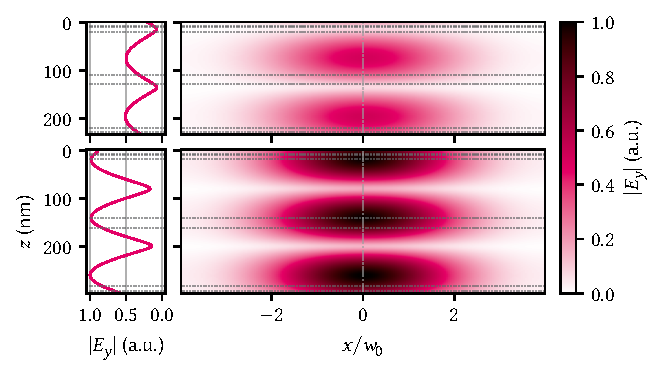
\includegraphics{img/pdf/experiment/tmm_field}
    \caption[\imgsource{img/py/experiment/tmm.py}]{
        Absolute value of the electric field inside the double-gated heterostructure under illumination with a Gaussian beam at $\lambda_0=\qty{825}{\nano\meter}$ from the top.
        Top (bottom) panels show the structure with the default (optimized) barrier thickness of \qty{90}{\nano\meter} (\qty{122}{\nano\meter}), respectively.
        Dotted horizontal lines indicate interfaces between different materials while the vertical dash-dotted line indicates the position of the line cuts shown in the left column.
        Increasing the thickness of the barrier has two beneficial effects; first, the overall field intensity inside the structure is higher by a factor of two, and second, there is a peak rather than a knot in the \gls{qw} at a depth of $\sim\qty{120}{\nano\meter}$ ($\sim\qty{150}{\nano\meter}$), leading to enhanced absorption.
    }
    \label{fig:exp:tmm:field}
\end{figure}

\begin{marginfigure}
    \centering
    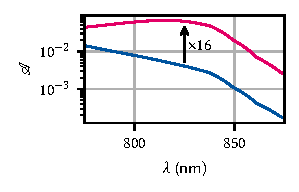
\includegraphics{img/pdf/experiment/tmm_absorptance}
    \caption[\imgsource{img/py/experiment/tmm.py}]{
        \Gls{qw} absorptance \absorptance in a heterostructure with default (blue) and optimized (magenta) barrier thickness and top and bottom gates as function of wavelength.
        Optimization was performed at \qty{825}{\nano\meter} using the differential evolution algorithm implemented in \pymoosh, resulting in a barrier thickness of \qty{122}{\nano\meter} and an absorptance better by a factor of \num{16} at \qty{6.3}{\percent}.
    }
    \label{fig:exp:tmm:wavelengths}
\end{marginfigure}

\Cref{fig:exp:tmm:wavelengths} depicts the absorptance at the optimal barrier thickness of \qty{122}{\nano\meter} as function of incident wavelength $\lambda_0$.
\absorptance is enhanced by a factor of up to \num{16} over a broad wavelength range compared to the unoptimized case.
The resulting barrier thickness is only moderately larger than before and should still be thin enough to allow for sufficiently strong electric fields at moderate voltages.
The electric field distribution inside the membrane for illumination by a Gaussian beam with waist radius $w_0 = \qty{624}{\nano\meter}$ (\cref{part:setup}) computed according to \cref{eq:exp:tmm:gauss:x} is shown in \cref{fig:exp:tmm:field} for the (un)optimized case in the (top) bottom panels.
The left panels show a line cut taken at $x=0$.
As argued qualitatively above, in the case of a thinner barrier, the field displays a node at the \gls{qw} position indicated by dashed lines at a depth of $z=\qtylist[list-units = single]{100;120}{\nano\meter}$.
Conversely, the situation is reversed for the \qty{30}{\nano\meter} thicker barrier, which hosts a field maximum at the depth of the \gls{qw}.

\subsection{Field emission}\label{subsec:exp:tmm:green}
\begin{figure*}
    \centering
    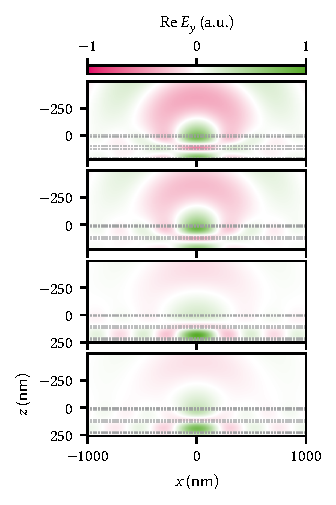
\includegraphics{img/pdf/experiment/tmm_green}
    \caption[\imgsource{img/py/experiment/tmm.py}]{
        Real part of the electric field emitted by a current line located in the \gls{qw} (black point) for different cases of the unoptimized (top row) and optimized (bottom row) structures.
        Left column shows the bare structures, right the double-gated ones.
        The half space $z<0$ is the air above the membrane in the direction of the objective lens and the dotted lines indicate interfaces between materials.
        Evidently, the gates reduce the amplitude in the upper half of the membrane and thereby the outcoupling efficiency compared to the bare structure, consistent with what is observed in the experiment.
        Optimizing the barrier thickness for absorption in the \gls{qw} drastically improves the outcoupling efficiency into the halfspace $z<0$ for both the bare and gated structures, although actually the latter (bottom right panel) radiates more power into the surface normal direction when compared with the ungated structure (bottom left).
    }
    \label{fig:exp:tmm:green}
\end{figure*}

So far, we have considered the absorption of the incident laser radiation in the \gls{qw}, a situation akin to placing the light source outside above the simulated structure.
To see how multilayer interference affects the extraction of light emitted \emph{inside} the structure, we turn to the Green's function calculation of \cref{eq:exp:tmm:helmholtz:green}.
That is, we place an infinitely long and in the $xz$ plane point-like current line in the center of the \gls{qw} to model the radiation emitted from a dipole.
Evidently, this is an approximation as the solution will have the same cylindrical symmetry as the source, whereas a more realistic model would contain a point-dipole producing a field distribution as described in \cref{subsec:setup:optics:coupling:efficiency}.
Nonetheless, in the plane of the point-dipole, the field should be well approximated by that of an infinitely long current line.
We once again use \pymoosh to perform the simulation.

\Cref{fig:exp:tmm:green} shows the real part of the electric field for two different geometries: the bare heterostructure (left column) and the double-gated structure (right column).
The source is indicated by a black dot and interfaces between different materials by dotted lines.
The top row shows the results for the unoptimized barrier thickness, where clearly the presence of the gates attenuates the outcoupling from the membrane into the air halfspace above ($z < 0$).
For the unoptimized, bare structure the emission pattern is close to cylindrical as would be the case in a homogeneous medium.
Increasing the barrier thickness (bottom left panel) in this case results in a complicated standing-wave pattern inside the membrane.
When adding the gates on both sides (bottom right panel), an emission pattern close to that of the unoptimized, bare structure is recovered, albeit with a higher extraction efficiency from the membrane.

These results demonstrate that on top of increasing the absorption efficiency, the extraction efficiency of \gls{pl} radiation from inside the membrane is further enhanced when increasing the \ch{AlGaAs} barrier thickness by a modest \qty{32}{\nano\meter}, leading us to expect an improvement larger than 16-fold in the end-to-end optical efficiency of \gls{pl} experiments.
